\subsection{Persona}
Abbiamo individuato e definito dettagliatamente sei \textit{persona}\footnote{Con il termine \textit{persona} si intende un utente sintetico ideato in modo che incarni tutte gli aspetti (intenzioni, obiettivi, attitudini, comportamenti, abitudini...) differenti che si vogliono supportare nell'ambito del design di un prodotto.}, ciascuna raffigurante un profilo interessante e peculiare. 

In una prima iterazione, nella selezione delle \textit{persona} avevamo incluso anche i giornalisti di testate esclusivamente online, per poi accorgerci che presentavano caratteristiche del tutto assimilabili alla \textit{persona} del blogger e del giornalista di testate nazionali o locali. \\ 
Inoltre, in una prima versione, avevamo selezionato la \textit{persona} "cittadino", ma, nel definirla, ci siamo accorti della possibilità di articolarla in due \textit{persona} distinte, quella del "cittadino esperto" e quella dell'"utente che utilizza smartphone".\\
Dall'analisi più approfondita delle dashboard presistenti, ci siamo resi conto della presenza importante di colori come strumento per distinguere gli elementi grafici: essendo per tali applicazioni web di assoluta rilevanza il "colpo d'occhio", crediamo che affidarsi solamente alla capacità distintiva dei colori sia insufficiente, considerando le persone affette da daltonismo. Pertanto, un'ulteriore iterazione ci ha portato a caratterizzare maggiormente la \textit{persona} Giulio, esplicitando la sua difficoltà nel riconoscere determinate tonalità.

Di seguito riportiamo le persona cui siamo giunti, articolandole per tipologia e presentando per ognuna una foto, un elenco puntato delle informazioni salienti richieste e una descrizione discorsiva.

\subsubsection*{Protagonisti}
\textbf{Giornalista testata nazionale}
\begin{itemize}
	\item Attitudine:
	\begin{itemize}
	\item esperto con tecnologie informatiche per cui richiede a suo supporto sistemi configurabili secondo le sue esigenze;
    \item è pignolo e esige che gli giungano informazioni in maniera rigorosa, tempestiva;
    \item è oberato di impegni, per cui ha necessità di essere supportato nel suo lavoro da strumenti altamente produttivi e affidabili;
    \end{itemize}
    \item Comportamento: per comprendere i dati della Covid-19, usa solo dashboard (no testi di articoli, interviste…) che siano:
	\begin{itemize}
	    \item agevoli nella comprensione,
	    \item affidabili nel funzionamento;
    \end{itemize}
	\item Obiettivi (\textit{end goals}): scrittura rapida di articoli riguardanti l'andamento dell'epidemia con dati ricavati da dashboard del DPC per fornire un'analisi significativa data-driven (guidata dai dati);
	\item Motivazione/life goals: fornire informazioni rigorose ai suoi lettori, con particolar attenzione all'analisi dei dati per permettere loro di comprendere approfonditamente la situazione nel contesto, così da prevenire allarmismi o sottostime del fenomeno;
	\item Obiettivi del sistema:
	\begin{itemize}
	    \item sistema di notifiche in caso di aggiornamento dei dati;
	    \item configurabilità interfaccia;
	    \item tracciabilità dei dati (data lineage);
    \end{itemize}
\end{itemize}

\begin{wrapfigure}{r}{8cm}
    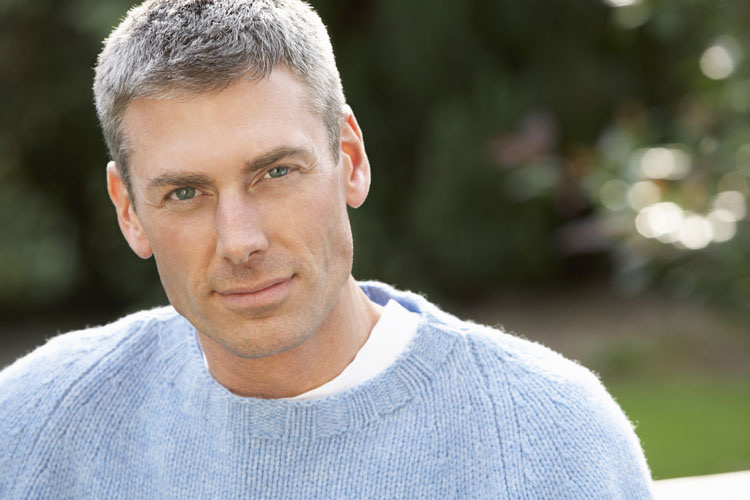
\includegraphics[scale=0.3]{studio-fattibilità/giovanni}
    \caption{Foto fantasiosa della persona Giovanni}
\end{wrapfigure}

Giovanni è un uomo di 53 anni di Fiumicino. È felicemente sposato da 24 anni e ha due figlie di 19 e 22 anni.
Dopo aver completato gli studi presso l'Università La Sapienza di Roma e aver fatto un po' di gavetta presso qualche giornale locale, lavora ormai da 19 anni presso "Il Corriere", dove ricopre il ruolo di redattore. Nell'ultimo anno si è occupato di scrivere articoli per informare i lettori sull'andamento dell'epidemia Covid-19. Ultimamente ha ripreso a lavorare in redazione assieme ad altre 10 persone, ognuno con la propria personale postazione correttamente distanziata dalle altre, formata da un computer fisso con un monitor 24".
Per scrivere i suoi articoli utilizza un software proprietario, sviluppato per l'azienda, di cui ormai conosce la maggior parte delle funzionalità. Nell'ultimo periodo ha imparato ad utilizzare la dashboard della Protezione Civile per ottenere i dati che inserisce nei suoi articoli.


\textbf{Giornalista testata locale}
\begin{itemize}
    \item Attitudine:
    \begin{itemize}
        \item approccio non rigoroso ai dati, per cui si fida delle dichiarazioni dei media pubblici e privati ritenuti affidabili;
        \item sguardo meno ampio sullo scenario nazionale ma ristretto alla propria realtà cittadina/regionale;
    \end{itemize}
	\item Comportamento: 
	\begin{itemize}
	    \item usa dashboard e legge articoli e dichiarazioni in Internet dei sindaci e presidente di regione;
		compresi l'andamento della pandemia, intervista sindaci e imprenditori locali per ascoltare le loro opinioni o prospettive future;
    \end{itemize}
	\item Obiettivi/end goals: raccontare come il Covid-19 abbia influenzato e continui a influenzare la realtà in cui vive e come il territorio reagisce,
	\begin{itemize}
        \item riflettendo sulle nuove sfide per la società (economiche, sociali…),
        \begin{itemize}
            \item sottolineando le criticità che possano coinvolgerli (chiusura piazze, corsi, centro commerciali…),
            \item pubblicizzando i contatti dei presidi sanitari/assistenziali locali e le buone pratiche da adottare;
        \end{itemize}
    \end{itemize}
	\item Motivazione/life goals: rendere i suoi concittadini consapevoli dell'evoluzione della pandemia nel loro territorio;
	\item Obiettivi del sistema:
    \begin{itemize}
        \item Possibilità di ricontestualizzare tutti gli elementi comunicativi dal livello nazionale a quello regionale (filtro per regione);
        \item Presentazione delle ordinanze regionali, con focus su quelle della regione di interesse;
    \end{itemize}
\end{itemize}

\begin{wrapfigure}{l}{8cm}
    
\includegraphics[scale=0.4]{studio-fattibilità/francesca}
    \caption{Foto fantasiosa della persona Francesca}
\end{wrapfigure}
        
Francesca è una donna di 36 anni di Mestre, laureatasi in Scienze della Comunicazione all'Università di Padova.
Lavora da sette anni presso la redazione del Gazzettino, in cui cerca di raccontare la propria regione e i suoi cittadini con passione, per fornire il proprio contributo diventato ancora più importante durante questa pandemia.
Essendo nella sua regione la situazione particolarmente critica, la direzione del giornale ha deciso di far lavorare da remoto e in presenza i suoi dipendenti a settimane alterne, mantenendo sempre invariati i gruppi che lavorano in presenza presso gli uffici in una determinata settimana in modo da poter prevenire delle possibili diffusioni del contagio. In redazione mantengono i contatti utilizzando strumenti di messaggistica come Slack, anche per mantenere i contatti lavorativi e non fra dipendenti degli stessi uffici.
Per via del suo percorso formativo e della passione per il suo territorio, ci tiene molto a raccontare ai propri concittadini come i numeri che tutti i giorni sentono per la televisione e leggono nei giornali modifichino le loro abitudini. Per questo motivo, oltre all'analisi dei dati provenienti dalla dashboard della Protezione Civile e dai bollettini regionali cerca quanto più possibile di intervistare i sindaci delle città venete per chiedere come si stanno muovendo per fronteggiare l'emergenza e a raccontare le attività svolte dagli imprenditori locali per aiutare il loro territorio.

\textbf{Giornalista testata d'agenzia}
Attitudine:
forma mentis caratterizzata da rigore nella verifica della veridicità delle fonti delle informazioni
predisposizione a lavorare in maniera rapida, altamente produttiva, disposto ad utilizzare strumenti tecnologici di automatizzazione
Comportamento: 
verifica sempre le fonti, ricostruendo il data lineage (ciclo di vita dei dati)
aggiorna tempestivamente eventuali dati errati/incompleti
Immediata valutazione di segnalazioni in arrivo da altri presidi di informazione (team di ricerca segnala supposti errori nella comunicazione/raccolta dati)
Obiettivi/end goals: comunicare in maniera puntuale e tempestiva i dati visualizzati nella dashboard
Motivazione/life goals: informare le altre testate giornalistiche circa dati veritieri e verificati, costituire per loro un punto di riferimento credibile e autorevole
Obiettivi del sistema:
notifiche
link alle fonti
template per automatizzare creazione articoli standard con inserimento dinamico dati e loro condivisione sui canali dedicate

\begin{wrapfigure}{r}{7cm}
    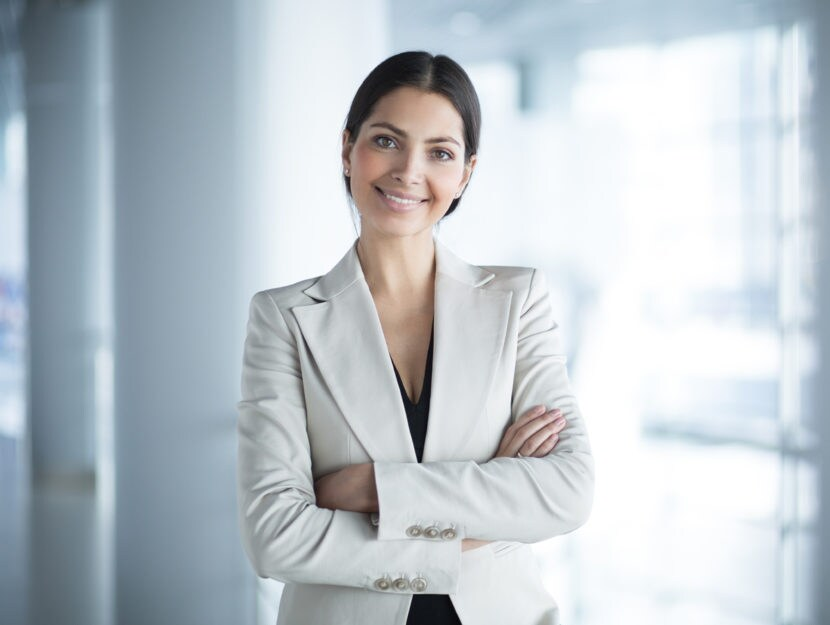
\includegraphics{studio-fattibilità/giulia}
    \caption{Foto fantasiosa della persona Giulia}
\end{wrapfigure}

Giulia è una donna di 35 anni, laureata in Scienze Politiche all'Università di Milano.
Grande appassionata di tecnologia, si informa su come essa possa semplificarle la vita: a casa ha infatti un'assistente vocale e le numerosi luci smart, controllabili tramite il suo smartphone.
Convive da otto anni con il suo fidanzato in un piccolo appartamento nel centro di Milano, a 10 minuti a piedi dall'ufficio dove lavora. Condivide l'ufficio assieme ad altre 4 persone, lavorando sul portatile datole dall'agenzia di stampa con il quale può lavorare anche da casa. L'agenzia richiede che il lavoro sia svolto principalmente in smart working finché la situazione non migliora, ma che se è necessario è possibile recarsi in ufficio.
Il suo ruolo nell'agenzia è quello di "fact-checking", ossia raccogliere i dati relativi ad un certo fenomeno e verificarne la veridicità, in modo che non vengano pubblicati dati errati o incompleti. 
Nell'ultimo periodo i dati che maggiormente ha studiato sono quelli relativi all'epidemia Covid-19. La sua fonte principale per questo tema è la dashboard della Protezione Civile ma fa riferimento in maniera rigorosa e sistematica anche alle fonti riferite in essa. Per il suo lavoro si trova spesso a ricostruire il ciclo di vita di ogni dato così da garantirne la veridicità. 
Per restare in comunicazione con i colleghi utilizza chat di gruppo, sistemi di collaborazione e file sharing, riuscendo a destreggiarsi con agevolezza tra le funzionalità che essi offrono. 

\subsubsection*{Persona secondarie}
\textbf{Opinionista/blogger}
	Attitudine:
		mentalità aperta;
		volontà di andare a fondo nelle notizie, raccogliendo pareri disparati;
	Comportamento: 
		lettura mattutina delle informazioni che continua a seguire nel resto della giornata mediante RSS
		interazione con i suoi follower, ascolto delle loro opinioni e raccolta sui cui creare nuovi contenuti che diano voce alla community o che siano ancor più interessanti per loro;
	Obiettivi/end goals: creare contenuti relativi all'epidemia, basando le sue argomentazioni sui dati della dashboard
	Motivazione/life goals: stimolare una libera discussione tra i suoi follower (lettori, ascoltatori…) sui temi caldi del momento
	Obiettivi del sistema:
		possibilità di esportare elementi grafici in formato immagine o widget HTML da incorporare;
		possibilità di selezionare solo alcuni elementi grafici per comporli in una mini dashboard da incorporare; 
		ogni grafico deve utilizzare modalità multiple per veicolare informazioni (mouse over per esplicitare contenuto informativo di componenti grafiche, icone…); 

\begin{wrapfigure}{l}{8cm}
    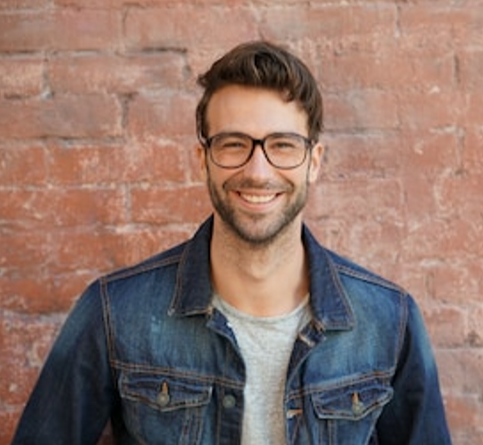
\includegraphics[scale=0.8]{studio-fattibilità/francesco}
    \caption{Foto fantasiosa della persona Francesco}
\end{wrapfigure}

Francesco è un uomo di 30 anni, che dopo aver terminato gli studi presso il liceo scientifico ha deciso di viaggiare in giro per l'Europa per un anno. Francesco è daltonico di tipo deuteranopico. Durante quest'anno ha conosciuto la sua attuale ragazza ed ora vivono assieme in un paesino vicino a Bellinzona. Francesco, grazie alle sue conoscenze informatiche ha creato un blog e ha aperto un canale YouTube. I contenuti che produce trattano di argomenti di attualità ed è seguito da un vasto pubblico di ragazzi tra i 16 e i 25 anni. Nel suo appartamento ha una stanza interamente  dedicata alla realizzazione dei video che poi pubblica sul suo canale YouTube, in questa stanza trova anche spazio una scrivania con 2 monitor da 27'' e un computer fisso di ultima generazione. Per aggiornare il suo blog utilizza Wordpress che ormai non ha più segreti per lui.
Da Marzo 2019 ha iniziato una rubrica settimanale nella quale racconta come si sta evolvendo la situazione in Italia e nel mondo per quanto riguarda l'epidemia Covid-19.  Il suo modus operandi è quello di seguire in maniera rigorosamente scientifica l'andamento dell'epidemia per offrire al suo pubblico una spiegazione ai difficili dati che i giornali divulgano. Utilizza diverse fonti per raccogliere e diversi strumenti per analizzare i dati. 

\subsubsection*{Persona addizionali}
\textbf{Cittadino esperto}
	Attitudine:
		voler aver voce nelle chiaccherate con amici
		voler contribuire ad un'informazione sana e corretta dei suoi familiari 
		ragionevole e responsabile, incline al rispetto delle istituzioni, fiducia nella scienza
	Comportamento: 
		Connessione alla dashboard sporadica, solo quando ha necessità di informarsi o ha ritagli di tempo libero
		condivide e discute delle informazioni acquisite con colleghi e amici
	Obiettivi/end goals:
		cercare di integrare quanto letto presso articoli di giornali di varia natura;
	Motivazione/life goals: acquisire maggiore consapevolezza e conoscenza dei fenomeni che impattano la realtà in cui vive, nonché la capacità di discernere l'essenziale dal mare magnum di informazioni che, continuamente, lo investono;
	Obiettivi del sistema:
		filtro per regione
		condivisione tramite mail/social network di una certa configurazione della dashboard per sostenere le sue riflessioni;
		grafica accattivante e grafici interattivi/configurabili

\begin{wrapfigure}{r}{8cm}
    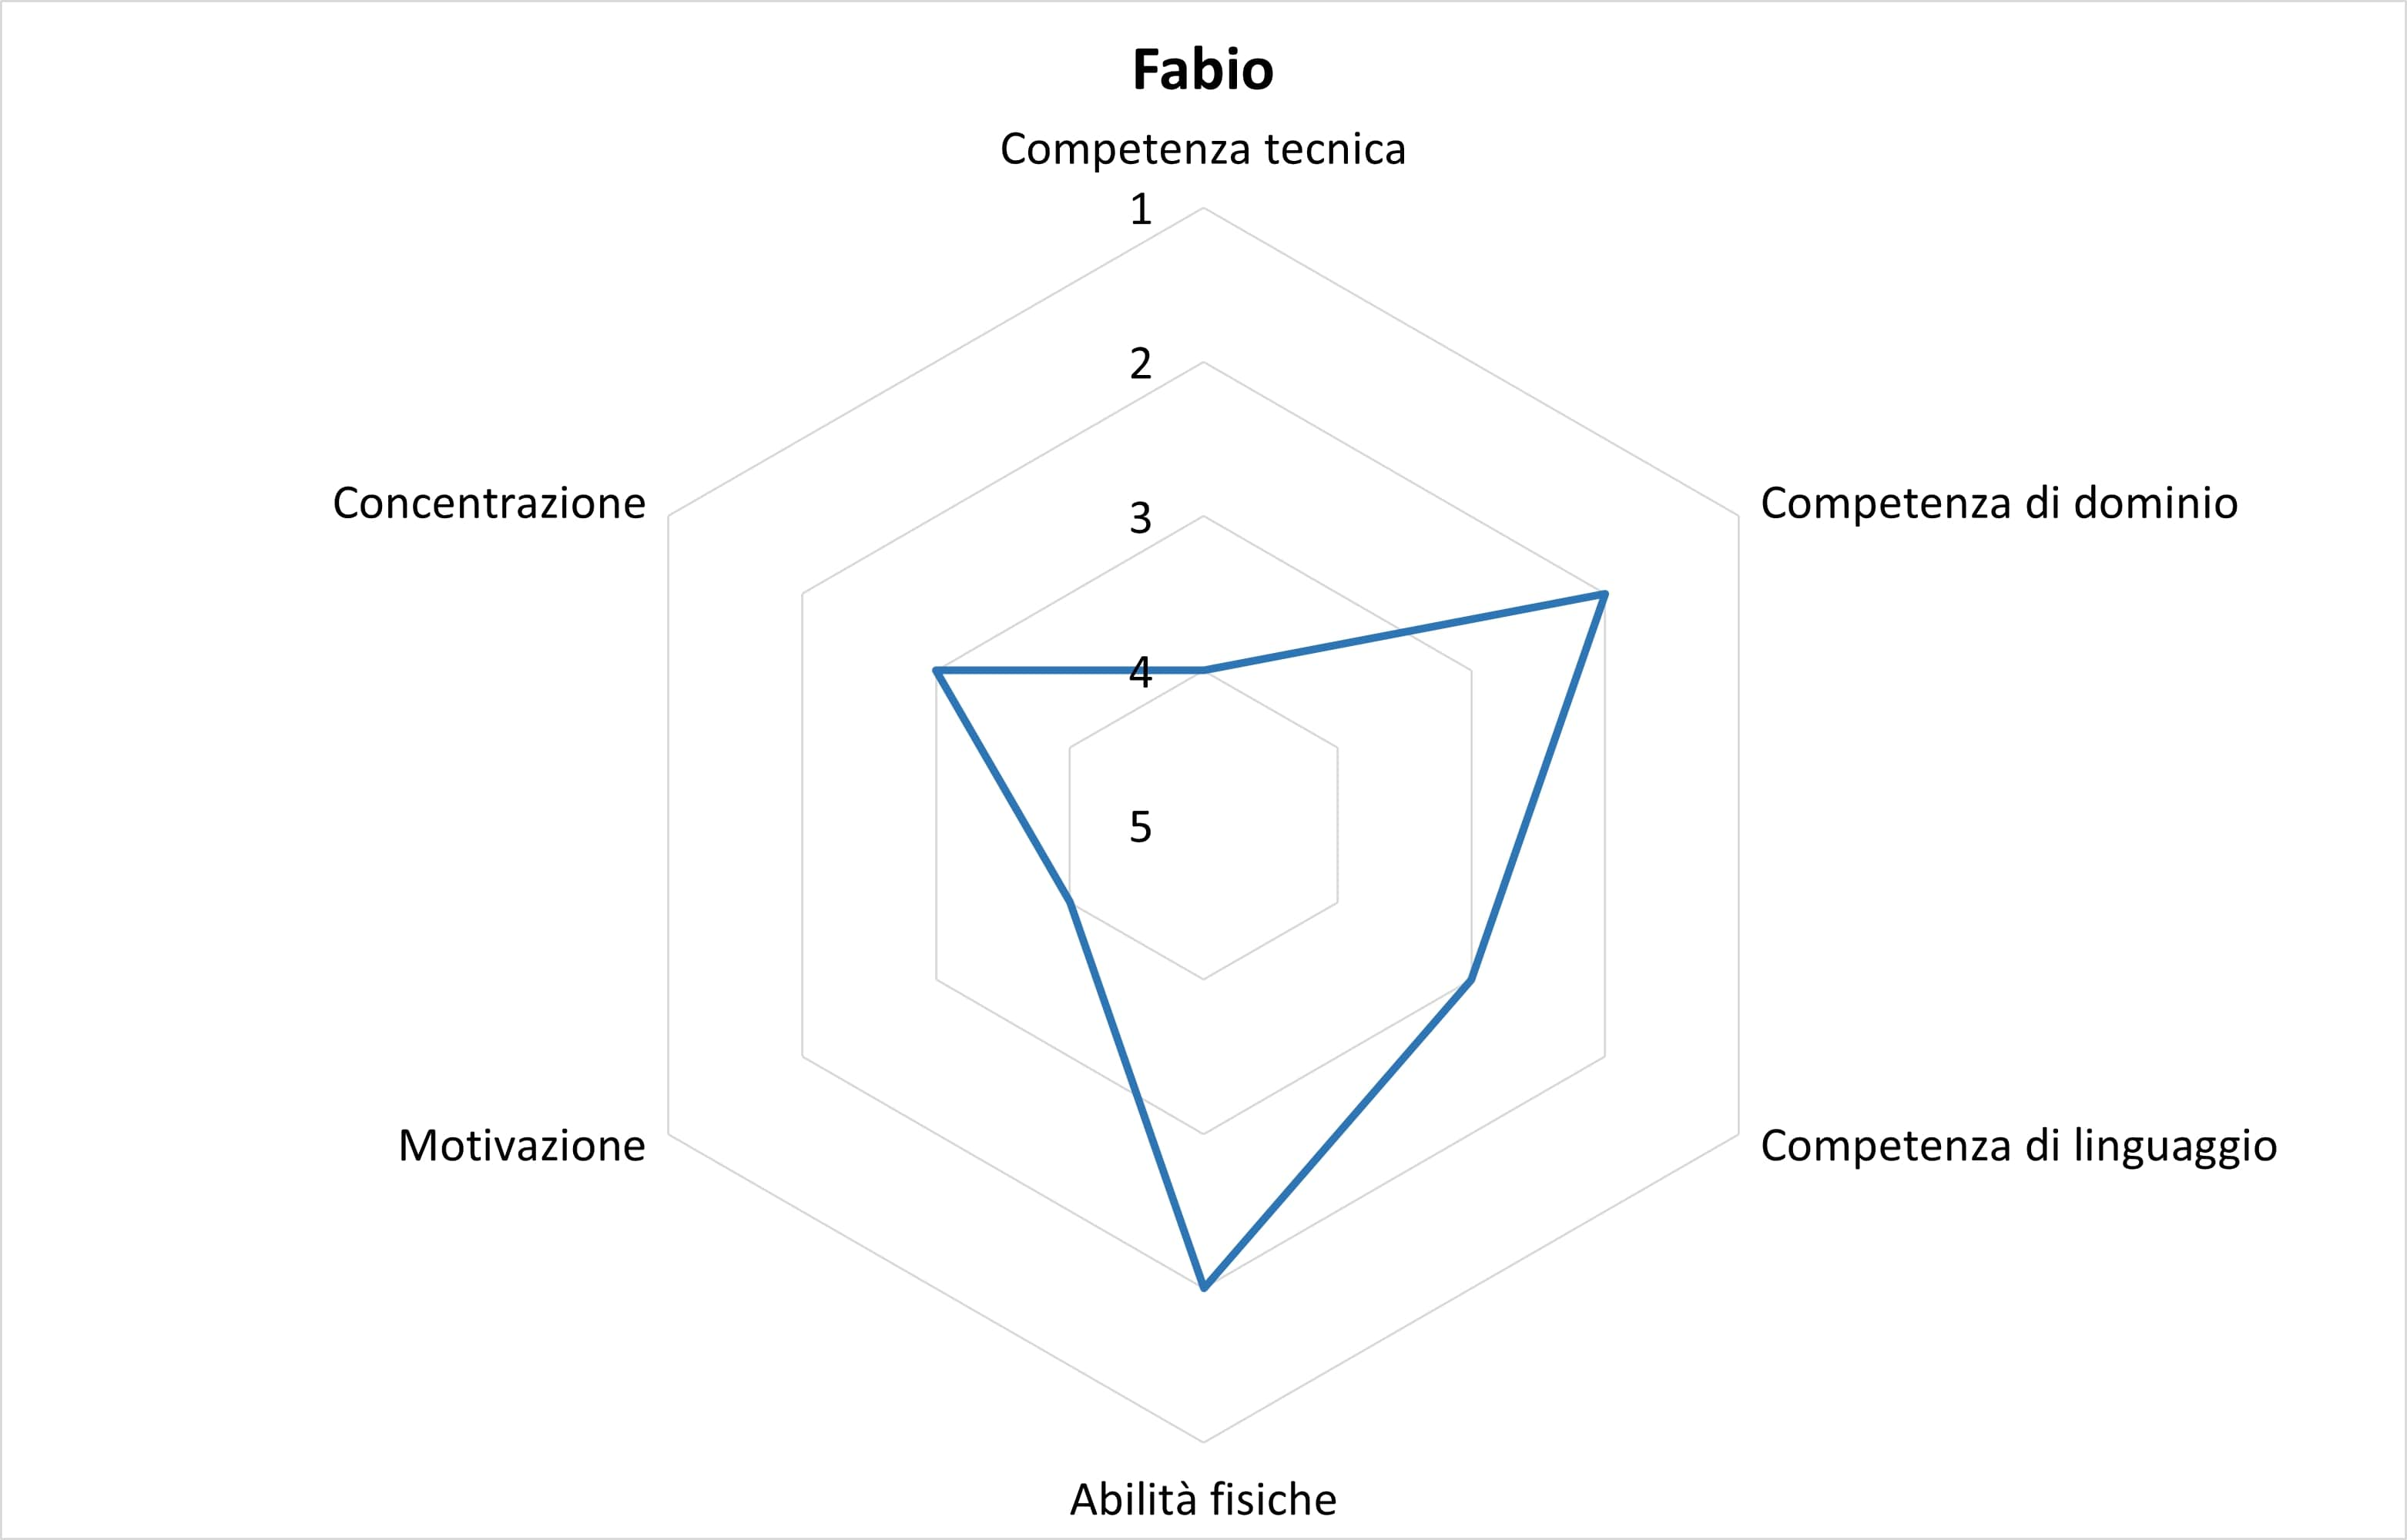
\includegraphics[scale=1.5]{studio-fattibilità/fabio}
    \caption{Foto fantasiosa della persona Fabio}
\end{wrapfigure}

Fabio è un uomo di 62 anni del Pescarese, la cui quotidianità è illuminata dalla sua famiglia e dal suo lavoro come docente universitario di Informatica presso l'Università degli Studi G. D'Annunzio (Chieti-Pescara).
E' sposato da 25 anni con Claudia, infermiera presso l'Ospedale S. Spirito di Pescara ed è padre di un'adolescente di 17 anni e un giovane di 23 anni: una delle abitudini più preziose della famiglia di Fabio è la condivisione della cena, durante la quale si parla delle attività di ognuno e si intavolano riflessioni circa le ultime notizie dall'Italia e dal mondo.
Negli anni, Fabio ha cercato di trasmettere ai figli il profondo rispetto che riconosce alle istituzioni, oltre alla fiducia che ripone nella scienza. Inoltre, è molto sensibile al dilagare delle fake news nei diversi ambiti: crede che siano responsabili di una cattiva informazione delle persone, e quindi di una loro consapevolezza distorta della realtà. 
Queste sue considerazioni emergono non solo in famiglia ma anche nei momenti di svago, ad esempio durante le chiaccherate con gli amici.
Ogni giorno, Fabio cerca di informarsi tramite canali considerati attendibili e autorevoli; negli ultimi mesi imperversati dalla pandemia Covid-19, ha esteso il suo briefing mattutino anche alla Dashbard della Protezione Civile: grazie alle sue competenze informatiche, riesce a consultarla in maniera agevole. In particolare, vi si rivolge quando gli articoli di giornale che legge si rivelano confusionari o non allineati: la dashboard presentando dati in maniera immediata permette a Fabio di dirimere i dubbi e acquisire l'essenziale; di frequente, estrae elementi grafici dalla dashboard per poi condividerli con i contatti dei suoi social, a corredo di proprie riflessioni.


\subsubsection*{Persona non-utenti, negative}
\textbf{Utente che utilizza lo smartphone per accedere alla dashboard}
	Attitudine:
		vita frenetica
		non un momento nella propria routine giornaliera per informarsi in maniera sistematica dal desktop
	Comportamento: 
		si informa con rassegne stampa
	Obiettivi/end goals: 
		fare ipotesi/ prevedere successive evoluzioni Covid e futuri provvedimenti governativi
	Motivazione/life goals: 
		informarsi sommariamente di quel che sta accadendo
	Obiettivi del sistema:
		piccolo testo che informa l'utente che la fruizione consigliata è attraverso desktop
ridurre le funzionalità al minimo per garantire accesso veloce e chiaro su schermi piccoli

\begin{wrapfigure}{l}{8cm}
    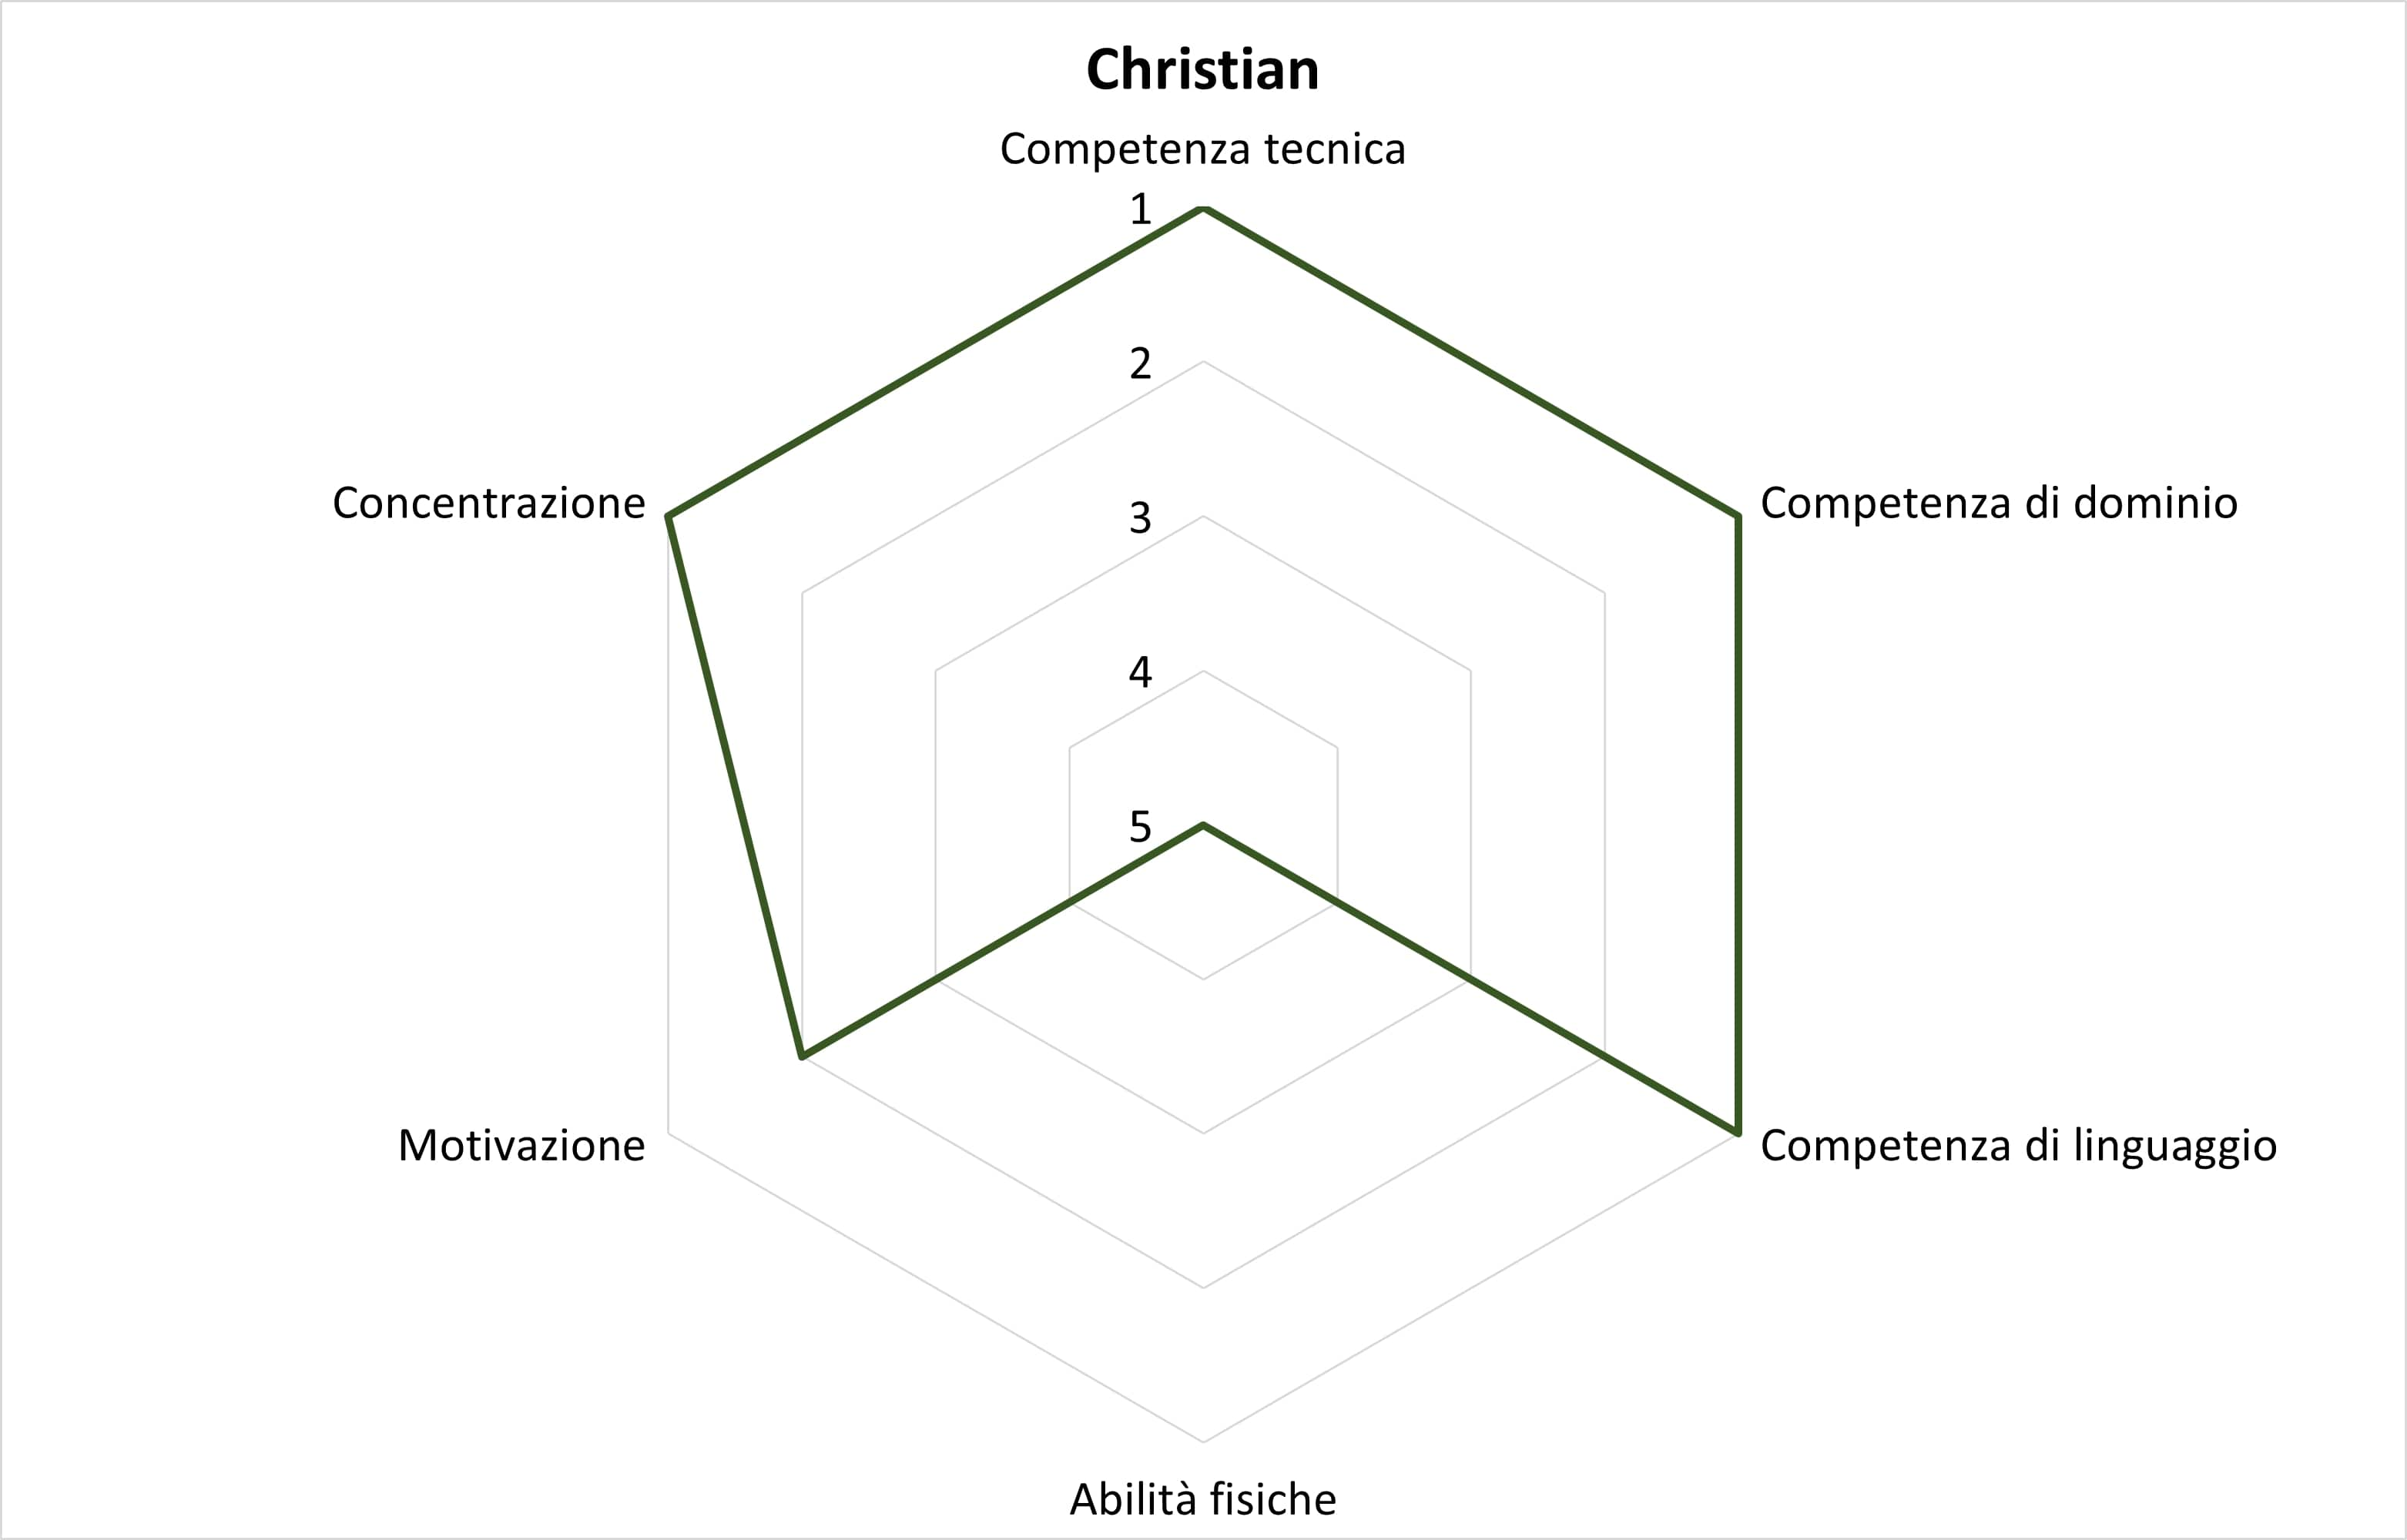
\includegraphics[scale=0.24]{studio-fattibilità/christian}
    \caption{Foto fantasiosa della persona Christian}
\end{wrapfigure}

Christian è un uomo di 34 anni che lavora come fattorino per un'agenzia di logistica.
Ha un appartamento a Torino vicino a una fermata della metropolitana e per raggiungere la propria sede di lavoro deve necessariamente prenderla quotidianamente. La sua giornata di lavoro inizia con la raccolta dei pacchi da consegnare durante l'arco della giornata con uno dei furgoni dell'azienda. L'impossibilità di muoversi per molte persone dovuta al lockdown e alla continua permanenza in smart working ha aumentato notevolmente i clienti dei negozi online e di conseguenza il lavoro di Christian ne ha risentito parecchio. Al ritorno a casa, la sera, non gli avanza molto tempo libero in quanto vive da solo e la casa se la deve gestire per conto proprio. Inoltre, la stanchezza lo porta a voler cercare di andare a dormire quanto prima, magari dopo essersi un po' riposato sul suo divano.
Nonostante il poco tempo a disposizione, ci tiene comunque a essere informato su ciò che avviene intorno a sé. Al mattino, prendendo la metropolitana, e in pausa pranzo, ascolta le rassegne stampa e legge alcuni giornali che ritiene affidabili, tra cui il Corriere, attraverso il suo smartphone con uno schermo da 6''. Se gli capita, legge anche il bollettino che l'ANSA ha pubblicato il giorno prima con i dati aggiornati sull'andamento dell'epidemia.


